\chapter{electromagnetic induction solutions}
\begin{abox}
	Practice set 1 solutions
	\end{abox}
\begin{enumerate}
\begin{minipage}{\textwidth}
	\item Consider a conducting loop of radius $a$ and total loop resistance $R$ placed in a region with a magnetic field $B$ thereby enclosing a flux $\phi_{0}$. The loop is connected to an electronic circuit as shown, the capacitor being initially uncharged\\
	\begin{figure}[H]
		\centering
		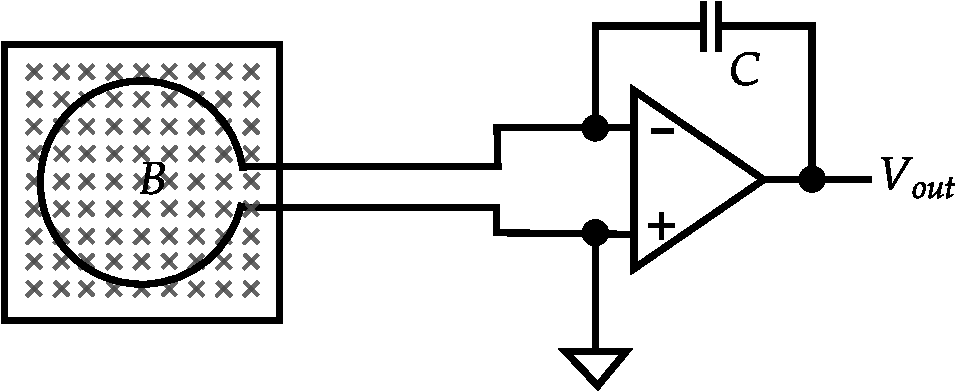
\includegraphics[height=3cm,width=5cm]{diagram-20210817(14)-crop}
	\end{figure}
	If the loop is pulled out of the region of the magnetic field at a constant speed $u$, the final output voltage $V_{\text {out }}$ is independent of
	\exyear{GATE 2010}
\end{minipage}
\begin{tasks}(4)
	\task[\textbf{A.}] $\phi_{0}$
	\task[\textbf{B.}]$u$ 
	\task[\textbf{C.}]$R$
	\task[\textbf{D.}] $C$ 
\end{tasks}
\begin{answer}
	The correct option is \textbf{(a)}	
\end{answer}
\begin{minipage}{\textwidth}
	\item A circular loop made of a thin wire has radius $2 \mathrm{~cm}$ and resistance $2 \Omega$. It is placed perpendicular to a uniform magnetic field of magnitude $\left|\vec{B}_{0}\right|=0.01$ Tesla. At time $t=0$ the field starts decaying as $\vec{B}=\vec{B}_{0} e^{-t / t_{0}}$, where $t_{0}=1 s .$ The total charge that passes through a cross section of the wire during the decay is $Q$. The value of $Q$ in $\mu C$ (rounded off to two decimal places) is
	\exyear{GATE 2019}
\end{minipage}
\begin{answer}
	\begin{align*}
	& \varepsilon=-\frac{d \phi}{d t}=-\frac{A d B}{d t}, I=\frac{\varepsilon}{R}=-\frac{d \phi}{d t} \frac{1}{R} \\
	&\Rightarrow-\frac{d \phi}{d t}=-\pi r^{2} \frac{d}{d t}\left(B_{0} e^{-t / t_{0}}\right)=\pi r^{2} B_{0} e^{-t}\left(t_{0}=1\right) \\
	&Q=\int_{0}^{\infty} I(t) d t=\int_{0}^{\infty} \frac{\pi r^{2}}{R} B_{0} e^{-t} d t=\frac{\pi r^{2} B_{0}}{R}\left|\frac{e^{-t}}{-1}\right|_{0}^{\infty} \\
	&=3.14 \times\left(2 \times 10^{-2}\right)^{2} \times 0.01=6.28 \mu C
	\end{align*}
\end{answer}
\begin{minipage}{\textwidth}
	\item A circular conducting ring of radius $R$ rotates with constant angular velocity $\omega$ about its diameter placed along the $x$-axis. A uniform magnetic field $B$ is applied along the $y$-axis. If at time $t=0$ the ring is entirely in the $x y$-plane, the emf induced in the ring at time $t>0$ is
	\exyear{JEST 2012}
\end{minipage}
\begin{tasks}(2)
	\task[\textbf{A.}] $B \omega^{2} \pi R^{2} t$
	\task[\textbf{B.}]$B \omega \pi R^{2} \tan (\omega t)$
	\task[\textbf{C.}]$B \omega \pi R^{2} \sin (\omega t)$
	\task[\textbf{D.}]$B \omega \pi R^{2} \cos (\omega t)$
\end{tasks}
\begin{answer}
	\begin{align*}
	&\phi_{m}=\vec{B} \cdot \vec{A}=B A \cos (90-\theta)=B A \sin \omega t\\
		&\varepsilon=-\frac{d \phi_{m}}{d t}=-\frac{d}{d t}(\vec{B} \cdot \vec{A})\\
		&=-\frac{d}{d t}[B A \sin \omega t]=-B A(\cos \omega t) \omega \\
		&\Rightarrow \varepsilon=-B \pi R^{2} \omega \cos \omega t \\
		& \varepsilon=B \omega \pi R^{2} \cos \omega t
	\end{align*}
	The correct option is \textbf{(d)}
\end{answer}
\begin{minipage}{\textwidth}
	\item Two parallel rails of a railroad track are insulated from each other and from the ground. The distance between the rails is 1 meter. A voltmeter is electrically connected between the rails. Assume the vertical component of the earth's magnetic field to the $0.2$ gauss. What is the voltage developed between the rails when a train travels at a speed of $180 \mathrm{~km} / \mathrm{h}$ along the track? Give the answer in milli-volts.
	\exyear{JEST 2018}
\end{minipage}
\begin{answer}
	$\text { Induced emf } \varepsilon=B l v=\left(0.2 \times 10^{-4}\right) \times 1 \mathrm{~m} \times 180 \times \frac{10}{60 \times 60}=10^{-3} \text { volts }=1 \mathrm{mV}$
\end{answer}
\begin{minipage}{\textwidth}
	\item A circular metal loop of radius $a=1 \mathrm{~m}$ spins with a constant angular velocity $\omega=20 \pi \mathrm{rad} / \mathrm{s}$ in a magnetic field $B=3$ Tesla, as shown in the figure. The resistance of the loop is 10 ohms. Let $P$ be the power dissipated in one complete cycle. What is the value of $\frac{P}{\pi^{4}}$ in Watts?
	\exyear{JEST 2019}
\end{minipage}
\begin{answer}
	\begin{align*}
	\text { Magnetic flux through the loop is }\\
	\phi_{m}&=\int_{S} \vec{B} d \vec{a}=B \times \pi a^{2} \times \cos \omega t\\
	\intertext{Induced e.m.f} \varepsilon&=-\frac{d \phi_{m}}{d t}=\omega B \times \pi a^{2} \times \sin \omega t\\.
	\intertext{Power dissipated} p&=\frac{\varepsilon^{2}}{R}=\frac{\omega^{2} B^{2} \pi^{2} a^{4} \sin ^{2} \omega t}{R}\\
	\intertext{Power dissipated in one complete cycle} P&=\langle p\rangle=\frac{\omega^{2} B^{2} \pi^{2} a^{4}}{2 R} \quad \because\left\langle\sin ^{2} \omega t\right\rangle=\frac{1}{2}\\
	\frac{P}{\pi^{4}}&=\frac{\omega^{2} B^{2} a^{4}}{2 \pi^{2} R} \Rightarrow P=\frac{(20 \pi)^{2}(3)^{2}(1)^{4}}{2(10)(10)}=18
	\end{align*}
\end{answer}
\end{enumerate}
\newpage
\begin{abox}
	Practice set 2 solutions
	\end{abox}
\begin{enumerate}
\begin{minipage}{\textwidth}
	\item A uniform magnetic field in the positive $z$-direction passes through a circular wire loop of radius $1 \mathrm{~cm}$ and resistance $1 \Omega$ lying in the $x y$-plane. The field strength is reduced from 10 tesla to 9 tesla in $1 s$. The charge transferred across any point in the wire is approximately
	\exyear{NET JUNE 2015}
\end{minipage}
\begin{tasks}(2)
	\task[\textbf{A.}]$3.1 \times 10^{-4}$ coulomb
	\task[\textbf{B.}] $3.4 \times 10^{-4}$ coulomb
	\task[\textbf{C.}] $4.2 \times 10^{-4}$ coulomb
	\task[\textbf{D.}]$5.2 \times 10^{-4}$ coulomb
\end{tasks}
\begin{answer}	
 \begin{align*}
 \varepsilon&=-\frac{d \phi}{d t} \Rightarrow I=\frac{d q}{d t}=\frac{\varepsilon}{R}=-\frac{1}{R} \frac{d \phi}{d t} \\
 d q&=-\frac{A}{R} d B=\frac{-\pi r^{2}}{R} d B \\
 d q&=\frac{-3.14 \times\left(10^{-2}\right)^{2}}{1} \times 1=3.14 \times 10^{-4} \text { coulomb }
 \end{align*}	
	The correct option is \textbf{(a)}	
\end{answer}
\begin{minipage}{\textwidth}
	\item A magnetic field $B$ is $B \hat{z}$ in the region $x>0$ and zero elsewhere. A rectangular loop, in the $x y$-plane, of sides $l$ (along the $x$-direction) and $h$ (along the $y$ - direction) is inserted into the $x>0$ region from the $x<0$ region at constant velocity $v=v \hat{x}$. Which of the following values of $l$ and $h$ will generate the largest EMF?
	\exyear{NET JUNE 2016}
\end{minipage}
\begin{tasks}(2)
	\task[\textbf{A.}] $l=8, h=3$
	\task[\textbf{B.}]$l=4, h=6$
	\task[\textbf{C.}]$l=6, h=4$
	\task[\textbf{D.}]$l=12, h=2$
\end{tasks}
\begin{answer}
	$\phi_{m} \propto B h x$
	$$
	\varepsilon \propto \frac{-d \phi_{m}}{d t} \propto B v h \propto h
	$$
	\begin{figure}[H]
		\centering
		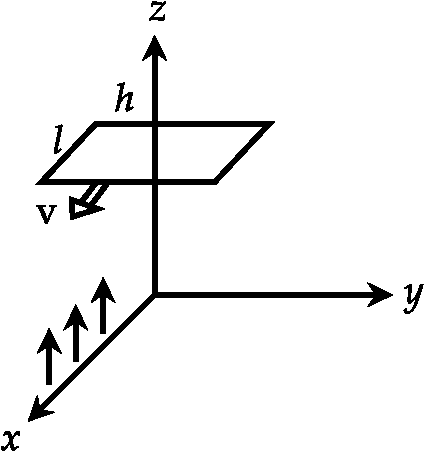
\includegraphics[height=3cm,width=5cm]{diagram-20211011(42)-crop}
	\end{figure}
	The correct option is \textbf{(b)}	
\end{answer}
\end{enumerate}